\documentclass{article}

% Language setting
% Replace `english' with e.g. `spanish' to change the document language
\usepackage[spanish]{babel}

% Set page size and margins
% Replace `letterpaper' with `a4paper' for UK/EU standard size
\usepackage[letterpaper,top=2cm,bottom=2cm,left=3cm,right=3cm,marginparwidth=1.75cm]{geometry}

% Useful packages
\usepackage{amsmath}
\usepackage{graphicx}
\usepackage{enumitem}
\usepackage{comment}
\usepackage{wrapfig}
\usepackage[colorlinks=true, allcolors=blue]{hyperref}

\title{Redes Tema 1. Introducción}
\author{Martín González Dios 
\href{https://github.com/martindios}{\includegraphics[height=0.5cm]{github.png}}}

\begin{document}
\maketitle

\section{Elementos de Internet}

\begin{figure}[h]
    \centering
    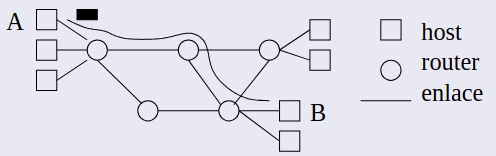
\includegraphics[width=0.5\textwidth]{img-t1/img_298_51.png}
    \caption{Representación de como funcionan los elementos de Internet}
\end{figure}

\subsection{Hardware}
\begin{itemize}
    \item \textbf{Hosts}: origen y destino de transmisiones (sistemas terminales).
    \item \textbf{Enlaces}: medios físicos por los que se realizan las transmisiones.
    \item \textbf{Routers}: dispositivos que interconectan enlaces.
\end{itemize}

\subsection{Software}
\begin{itemize}
    \item \textbf{Protocolos}: básicos(TCP/IP, UDP, ICMP, ...) y de aplicación(HTTP, SMTP, ...).
    \item \textbf{Proveedores de servicios de Internet} (ISP): de baja escala (residenciales, dan acceso a usuarios) o de alta escala (líneas de larga distancia, interconectan proveedores a baja escala, nacionales, ...).
\end{itemize}

\section{Servicio orientado a conexión}
\textbf{TCP}(Transmission Control Protocol).
\subsection{Fases}
\begin{enumerate}
    \item Establecimiento de la conexión (el usuario solicita una conexión, se fijan parámetros y se preparan ambos extremos para la transmisión).
    \item Transmisión de datos.
    \item Desconexión.
\end{enumerate}

\subsection{Características}
\begin{itemize}
    \item \textbf{Segmentación}: TCP recoge datos que la aplicación escribe en el socket y forma paquetes (MSS, tamaño máximo de segmento).
    \item \textbf{Transferencia fiable}: el receptor envía confirmaciones (ACK, Acknowledgment), si no se reciben se retransmite.
    \item \textbf{Control de flujo}: el receptor puede controlar la tasa de envío del emisor (mecanismo de TCP).
    \item \textbf{Control de congestión}: permite que la tasa de envío se ajuste a las capacidades de la red.
\end{itemize}

\section{Servicio no orientado a conexión}
\textbf{UDP}(User Datagram Protocol).
\begin{itemize}
    \item No hay fase de establecimiento de conexión.
    \item No hay confirmaciones: el emisor desconoce si el paquete llegó al destino.
    \item No hay control de flujo ni de congestión.
    \item La \textbf{transmisión es más rápida, pero menos fiable}.
\end{itemize}

\section{Tipos de redes}
\subsection{Conmutación}
\textbf{Llegan por un lado y salen por otro}, son circuitos (pueden ser sin multiplexación, FDM [multiplexación por división de frecuencia] o TDM [multiplexación por división de tiempo]) y paquetes (pueden ser datagramas o circuitos virtuales).

\subsection{Difusión}
\textbf{Todos los hosts reciben las transmisiones}, pero solo el destinatario la procesa, un ejemplo sería Ethernet.


\section{Redes de conmutación de circuitos}
\begin{figure}[h]
    \centering
    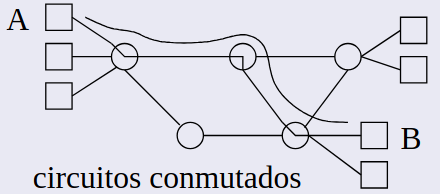
\includegraphics[width=0.3\textwidth]{img-t1/img_325_50.png}
\end{figure}

\begin{enumerate}
    \item \textbf{Fase de conexión} en la que se reservan recursos hardware. No pueden ser usados por otra transmisión. Se establece la ruta que van a seguir los datos. Ranuras temporales (TDM) o bandas de frecuencia (FDM).
    \item \textbf{Transmisión de datos}.
    \item \textbf{Fase de desconexión}: se liberan todos los recursos.
\end{enumerate}
Las redes de conmutación de circuitos \textbf{derrochan recursos}, pues los reserva aunque la transmisión no los use.

\newpage

\section{Redes de Conmutación de Paquetes}

En las \textbf{redes de conmutación de paquetes}, no se reservan recursos para cada conexión, sino que estos se \textbf{comparten} y se \textbf{asignan bajo demanda}. Estas redes trabajan con \textbf{paquetes} (segmentación), los cuales contienen una cabecera con información de control, como por ejemplo los \textbf{ACK}. Los \textbf{routers} son un ejemplo de conmutadores de paquetes que funcionan mediante el modelo \textbf{store-and-forward}, en el cual reciben un paquete, lo almacenan en una cola y luego lo reenvían. Si la cola está llena, el paquete es descartado.

\subsection{Tipos de Retardos}
Los retardos en este tipo de redes se clasifican en:
\begin{itemize}
    \item \textbf{Retardo de procesamiento:} Es el tiempo necesario para examinar la cabecera y dirigir el paquete a la salida correspondiente.
    \item \textbf{Retardo de espera en la cola:} Este retardo es proporcional a la carga de la red y depende del tiempo que el paquete permanece en la cola antes de ser procesado.
    \item \textbf{Retardo de transmisión:} Se calcula como la longitud del paquete dividida entre la tasa de transmisión.
    \item \textbf{Retardo de propagación:} Se calcula como la longitud del enlace dividida entre la velocidad de propagación.
\end{itemize}

El \textbf{retardo total} es la suma de todos estos retardos. Por su parte, el \textbf{retardo de extremo a extremo} es la suma de los retardos de todos los saltos en el camino del paquete. Si el emisor espera \textbf{ACKs}, se considera el \textbf{RTT} (Round Trip Time), que corresponde al doble del retardo.

\subsection{Capacidad y Aprovechamiento del Enlace}
\begin{itemize}
    \item La \textbf{capacidad del enlace} (cantidad máxima de bits que podrían estar en tránsito en un momento dado) se calcula como el producto del \textbf{retardo} por el \textbf{ancho de banda}.
    \item El \textbf{aprovechamiento del enlace} es la cantidad de bits que el emisor debe transmitir antes de que llegue el primer bit al receptor.
\end{itemize}

\subsection{Segmentación}
La segmentación tiene varias ventajas:
\begin{itemize}
    \item Reduce el tiempo de transmisión.
    \item Evita la saturación de la red.
    \item Permite intercalar conexiones.
    \item Si hay errores, solo se retransmiten los paquetes afectados.
\end{itemize}

\newpage

\subsection{Tipos de Conmutación de Paquetes}
Existen dos tipos principales de conmutación de paquetes:
\begin{itemize}
    \item \textbf{Datagramas}
    \begin{itemize}
        \item No están orientadas a conexión.
        \item El encaminamiento se realiza en función del destino (cabecera del paquete = IP destino).
        \item Cada router reenvía el paquete según la información de su tabla de reenvío.
        \item Los routers no mantienen información de estado, por lo que varios paquetes con la misma IP pueden ser encaminados de forma independiente.
    \end{itemize}
    \item \textbf{Circuitos Virtuales}
    \begin{itemize}
        \item Están orientadas a conexión.
        \item El encaminamiento se realiza en función del número del circuito virtual (CV).
        \item Antes de la transmisión, se establece una conexión con una ruta planificada, asignándose un número de circuito virtual.
        \item A cada paquete se le escribe el CV correspondiente, que los routers usan para su reenvío.
        \item Los routers mantienen información de estado en la tabla de circuitos virtuales.
    \end{itemize}
\end{itemize}

\newpage

\section{Acceso a Internet}

El acceso a Internet puede clasificarse en tres grandes categorías: acceso residencial, acceso empresarial y doméstico, y acceso móvil.

\subsection{Acceso residencial}
El acceso residencial incluye tecnologías como módem, DSL, cable HFC y FTTH:
\begin{itemize}
    \item \textbf{Módem}: Utiliza la línea telefónica como si fuese una llamada de voz. Este dispositivo establece la conexión llamando al número telefónico del proveedor de servicios de Internet (ISP). Además, realiza las siguientes funciones:
    \begin{itemize}
        \item \textit{Modulación}: Convierte la señal digital en una señal modulada para su transmisión.
        \item \textit{Desmodulación}: El receptor realiza la conversión inversa para interpretar la señal.
    \end{itemize}
    El ancho de banda disponible es muy estrecho, aproximadamente 4 kHz, lo que permite una velocidad máxima de transmisión de 56 kbps.
    
    \item \textbf{DSL (Digital Subscriber Line)}: Utiliza todo el ancho de banda de frecuencias del cable telefónico, que puede alcanzar hasta 1 MHz, logrando velocidades de transmisión de hasta 30 Mbps. Este sistema emplea \textit{Frequency Division Multiplexing} (FDM) para dividir la señal en tres canales:
    \begin{itemize}
        \item Canal de voz telefónica.
        \item Canal de subida para transmitir datos hacia Internet.
        \item Canal de bajada para recibir datos desde Internet.
    \end{itemize}
    
    \item \textbf{Cable HFC (Híbrido de Fibra y Coaxial)}: Este tipo de conexión utiliza una infraestructura combinada de fibra óptica y cable coaxial. Su estructura comprende:
    \begin{itemize}
        \item \textit{Cabecera final}: Centraliza las transmisiones de datos.
        \item \textit{Líneas troncales}: Conectan las cabeceras con los nodos.
        \item \textit{Ramales}: Distribuyen servicios como televisión, telefonía e Internet a los usuarios finales.
    \end{itemize}
    
    \item \textbf{FTTH (Fiber To The Home)}: Consiste en el uso de fibra óptica para la distribución de servicios avanzados, como el \textit{Triple Play} (Internet, televisión y telefonía). Su infraestructura incluye:
    \begin{itemize}
        \item \textit{OLT (Optical Line Terminal)}: Es el punto final que conecta con el ISP.
        \item \textit{ODN (Optical Distribution Network)}: Red que conecta el OLT con los usuarios.
        \item \textit{ONT (Optical Network Terminal)}: Convierte señales ópticas en señales eléctricas y viceversa.
    \end{itemize}
\end{itemize}

\subsection{Acceso empresarial y doméstico}
El acceso empresarial y doméstico utiliza redes locales (\textit{Local Area Networks}, LAN) basadas en tecnologías como Ethernet. Estas redes suelen estar conectadas a un enrutador (\textit{router}) que proporciona conexión a Internet mediante un enlace dedicado, separado de la línea telefónica convencional.

\subsection{Acceso móvil}
El acceso móvil incluye tecnologías como WiFi, 3G, 4G, LTE y 5G, permitiendo conexión inalámbrica a Internet desde dispositivos móviles. Esta forma de acceso combina flexibilidad y movilidad, siendo fundamental en entornos personales y laborales.

\newpage

\section{Medios de Transmisión}

Los medios de transmisión se clasifican en dos grandes categorías: \textit{medios guiados} y \textit{medios no guiados}.

\subsection{Medios guiados}
Los medios guiados conducen las señales a través de un medio físico, como cables. Entre ellos se encuentran:
\begin{itemize}
    \item \textbf{Cable de cobre de par trenzado}: Utiliza dos o más hilos de cobre trenzados para reducir interferencias electromagnéticas. Existen diferentes aplicaciones y configuraciones:
    \begin{itemize}
        \item \textit{Tipo telefónico}: Utiliza dos hilos trenzados.
        \item \textit{LAN}: Utiliza cuatro pares de hilos trenzados.
        \item \textit{UTP (Unshielded Twisted Pair)}: Categorías comunes como 5a y 6a, ampliamente utilizadas en redes.
        \item \textit{STP (Shielded Twisted Pair)}: Incluye blindaje para reducir interferencias.
    \end{itemize}
    
    \item \textbf{Cable coaxial}: Está compuesto por un núcleo de cobre, un aislante dieléctrico, una malla conductora y una capa externa de plástico. Este diseño minimiza las pérdidas de energía por radiación. Se distingue entre:
    \begin{itemize}
        \item \textit{50 $\Omega$}: Usado para señales sin modular.
        \item \textit{75 $\Omega$}: Utilizado en señales de banda ancha, como en redes HFC.
    \end{itemize}
    
    \item \textbf{Fibra óptica}: Transmite datos mediante pulsos de luz, evitando pérdidas por radiación e interferencias. Está fabricada con materiales transparentes que presentan baja atenuación, permitiendo transmisiones de hasta 100 km sin necesidad de repetidores. Sin embargo, su instalación es costosa y compleja. Existen dos tipos principales de fibra:
    \begin{itemize}
        \item \textit{Fibra multimodo}: La luz se propaga rebotando en las paredes del núcleo. Es utilizada en conexiones locales, centros de datos y aplicaciones como FTTH.
        \item \textit{Fibra monomodo}: La luz se propaga en línea recta, permitiendo mayores distancias, aunque a un costo más elevado.
    \end{itemize}
    Además, la designación \textit{OC-n} se utiliza para representar la velocidad de enlace, donde $n \times 51.8$ Mbps define la capacidad.
\end{itemize}

\subsection{Medios no guiados}
Los medios no guiados no requieren un medio físico sólido, ya que utilizan la atmósfera o el espacio como canal de transmisión. Entre ellos destacan:
\begin{itemize}
    \item \textit{Canales de radio terrestre}.
    \item \textit{Canales vía satélite}.
\end{itemize}

\newpage

\section{Arquitectura en Capas}

La arquitectura en capas \textbf{facilita el diseño de protocolos de comunicación dividiendo la comunicación en tareas específicas}, donde cada tarea se asigna a una capa independiente. Esta modularización permite que las capas superiores utilicen los servicios proporcionados por las capas inferiores, siempre respetando las especificaciones de cada capa. Entre las arquitecturas más conocidas se encuentran el modelo \textit{OSI} y \textit{TCP/IP}.

\subsection{Principios de la Arquitectura en Capas}
\begin{itemize}
    \item Cada capa realiza \textbf{tareas específicas} y está diseñada para ser independiente de las demás.
    \item Las capas superiores dependen de los servicios proporcionados por las capas inferiores.
    \item Este \textbf{diseño modular} simplifica el desarrollo, mantenimiento y escalabilidad de los protocolos de comunicación.
\end{itemize}

\subsection{Arquitectura TCP/IP}
La arquitectura \textit{TCP/IP} es una de las más utilizadas en las redes modernas. Divide la comunicación en cinco capas principales, cada una con funciones específicas:

\begin{enumerate}
    \item \textbf{Capa de Aplicación}: 
    \begin{itemize}
        \item Genera los mensajes.
        \item Localiza los procesos que se comunican por medio de mensajes.
        \item Ejemplos de protocolos: \textit{HTTP}, \textit{FTP}, \textit{SMTP}.
    \end{itemize}
    
    \item \textbf{Capa de Transporte (segmento)}:
    \begin{itemize}
        \item Prepara los mensajes para ser transmitidos fuera del ordenador.
        \item Recoge los datos del origen y forma paquetes.
        \item En el destino, comprueba que todos los datos han llegado correctamente y reensambla el mensaje.
        \item Protocolos comunes: \textit{TCP}, \textit{UDP}.
    \end{itemize}
    
    \item \textbf{Capa de Red (datagrama)}:
    \begin{itemize}
        \item Se encarga de buscar rutas y enviar paquetes entre los diferentes hosts.
        \item Utiliza protocolos de encaminamiento para determinar las rutas óptimas.
        \item Elemento principal: \textit{routers}.
    \end{itemize}
    
    \item \textbf{Capa de Enlace (trama)}:
    \begin{itemize}
        \item Transmite bloques de datos (tramas) a través de un enlace físico.
        \item Maneja detalles de bajo nivel, dependiendo de la tecnología de red utilizada (difusión, circuitos virtuales, etc.).
    \end{itemize}
    
    \item \textbf{Capa Física}:
    \begin{itemize}
        \item Convierte los bits en señales eléctricas, ópticas o inalámbricas.
        \item Define las características físicas del medio de transmisión, como el tipo de cable o frecuencia utilizada.
    \end{itemize}
\end{enumerate}

\subsection{Proceso de Encapsulación}
En la arquitectura \textit{TCP/IP}, \textbf{cada capa añade una cabecera} (información de control) al mensaje original, adaptándolo a sus propias funciones. A medida que el mensaje pasa por cada capa, su nombre cambia:
\begin{itemize}
    \item \textit{Mensaje}: Generado por la capa de aplicación.
    \item \textit{Segmento}: Procesado en la capa de transporte.
    \item \textit{Datagrama}: Manipulado en la capa de red.
    \item \textit{Trama}: Gestionado en la capa de enlace.
    \item \textit{Señal}: Convertido en la capa física para la transmisión.
\end{itemize}




\begin{comment}
\begin{figure}[h]
    \centering
    \includegraphics[width=0.5\textwidth]{1.png}
    \caption{}
\end{figure}
\end{comment}

\begin{comment}
\begin{wrapfigure}[]{r}{0.5\linewidth}
    \centering
    \includegraphics[width=\linewidth]{8.png}
    \caption{}
\end{wrapfigure}
\end{comment}

\end{document}